\section{Overview}
我们复现了De Cristofaro等人的高效PSI协议,并在此基础上进行改进,编写了基于证书的APSI协议的代码。代码仓库位于\href{https://github.com/Layotiver/apsi}
{https://github.com/Layotiver/apsi}。

我们基于了\textit{pycryptodome}包的哈希,取大质数,取随机数等功能,编程实现了扩展欧几里得算法,求乘法逆元,RSA公私钥生成,RSA加密等算法。这部分代码位于\textit{myutils.py}。

本次实验中,隐私集合的元素是英语单词,隐私集合求交即求出双方共有的单词。客户端和服务器端的单词分别保存在\textit{client\_set.txt}和\textit{server\_set.txt}中。其中客户端的单词为\textit{text, corpus, from, language, approach, resource},服务器端的单词为\textit{This, is, quite, a, departure, from, the, earlier, approach, in, NLP, applications}。其中\textit{from}和\textit{approach}是双方共有的单词。隐私集合求交的结果会输出这两个单词在Client集合里的下标,即2和4。对于哈希,我们使用sha256函数,并通过设置不同的salt值来产生不同的哈希函数。

\section{PSI protocol}
我们在\textit{psi}包里实现了De Cristofaro等人的PSI协议。其中\textit{Client}类和\textit{Server}类对于算法中的Client和Server。两个类都有\textit{off\_line}和\textit{on\_line}函数,对应协议中的离线和在线处理的部分。

运行\textit{main\_psi\_server.py}后,服务端程序启动。服务端会先进行\textit{off\_line}操作,然后监听本地的12121端口,接收来自客户端的PSI请求。接着运行\textit{main\_psi\_client.py},客户端先进行\textit{off\_line}操作,然后将协议中的需要传输的数据发送到本地的12121端口。服务器收到数据后进行一系列处理,即协议中的\textit{on\_line}部分,再发回处理过的数据给客户端。客户端收到数据后也进行\textit{on\_line}部分的操作,最后算出双方共有的集合元素。

运行\textit{main\_psi\_client.py}后,控制台打印出\textit{2,4},代表计算出隐私集合里第2个和第4个元素为共有的元素,结果正确,参见图\ref{fig:experiment0}。

\begin{figure}[t]
    \centering
    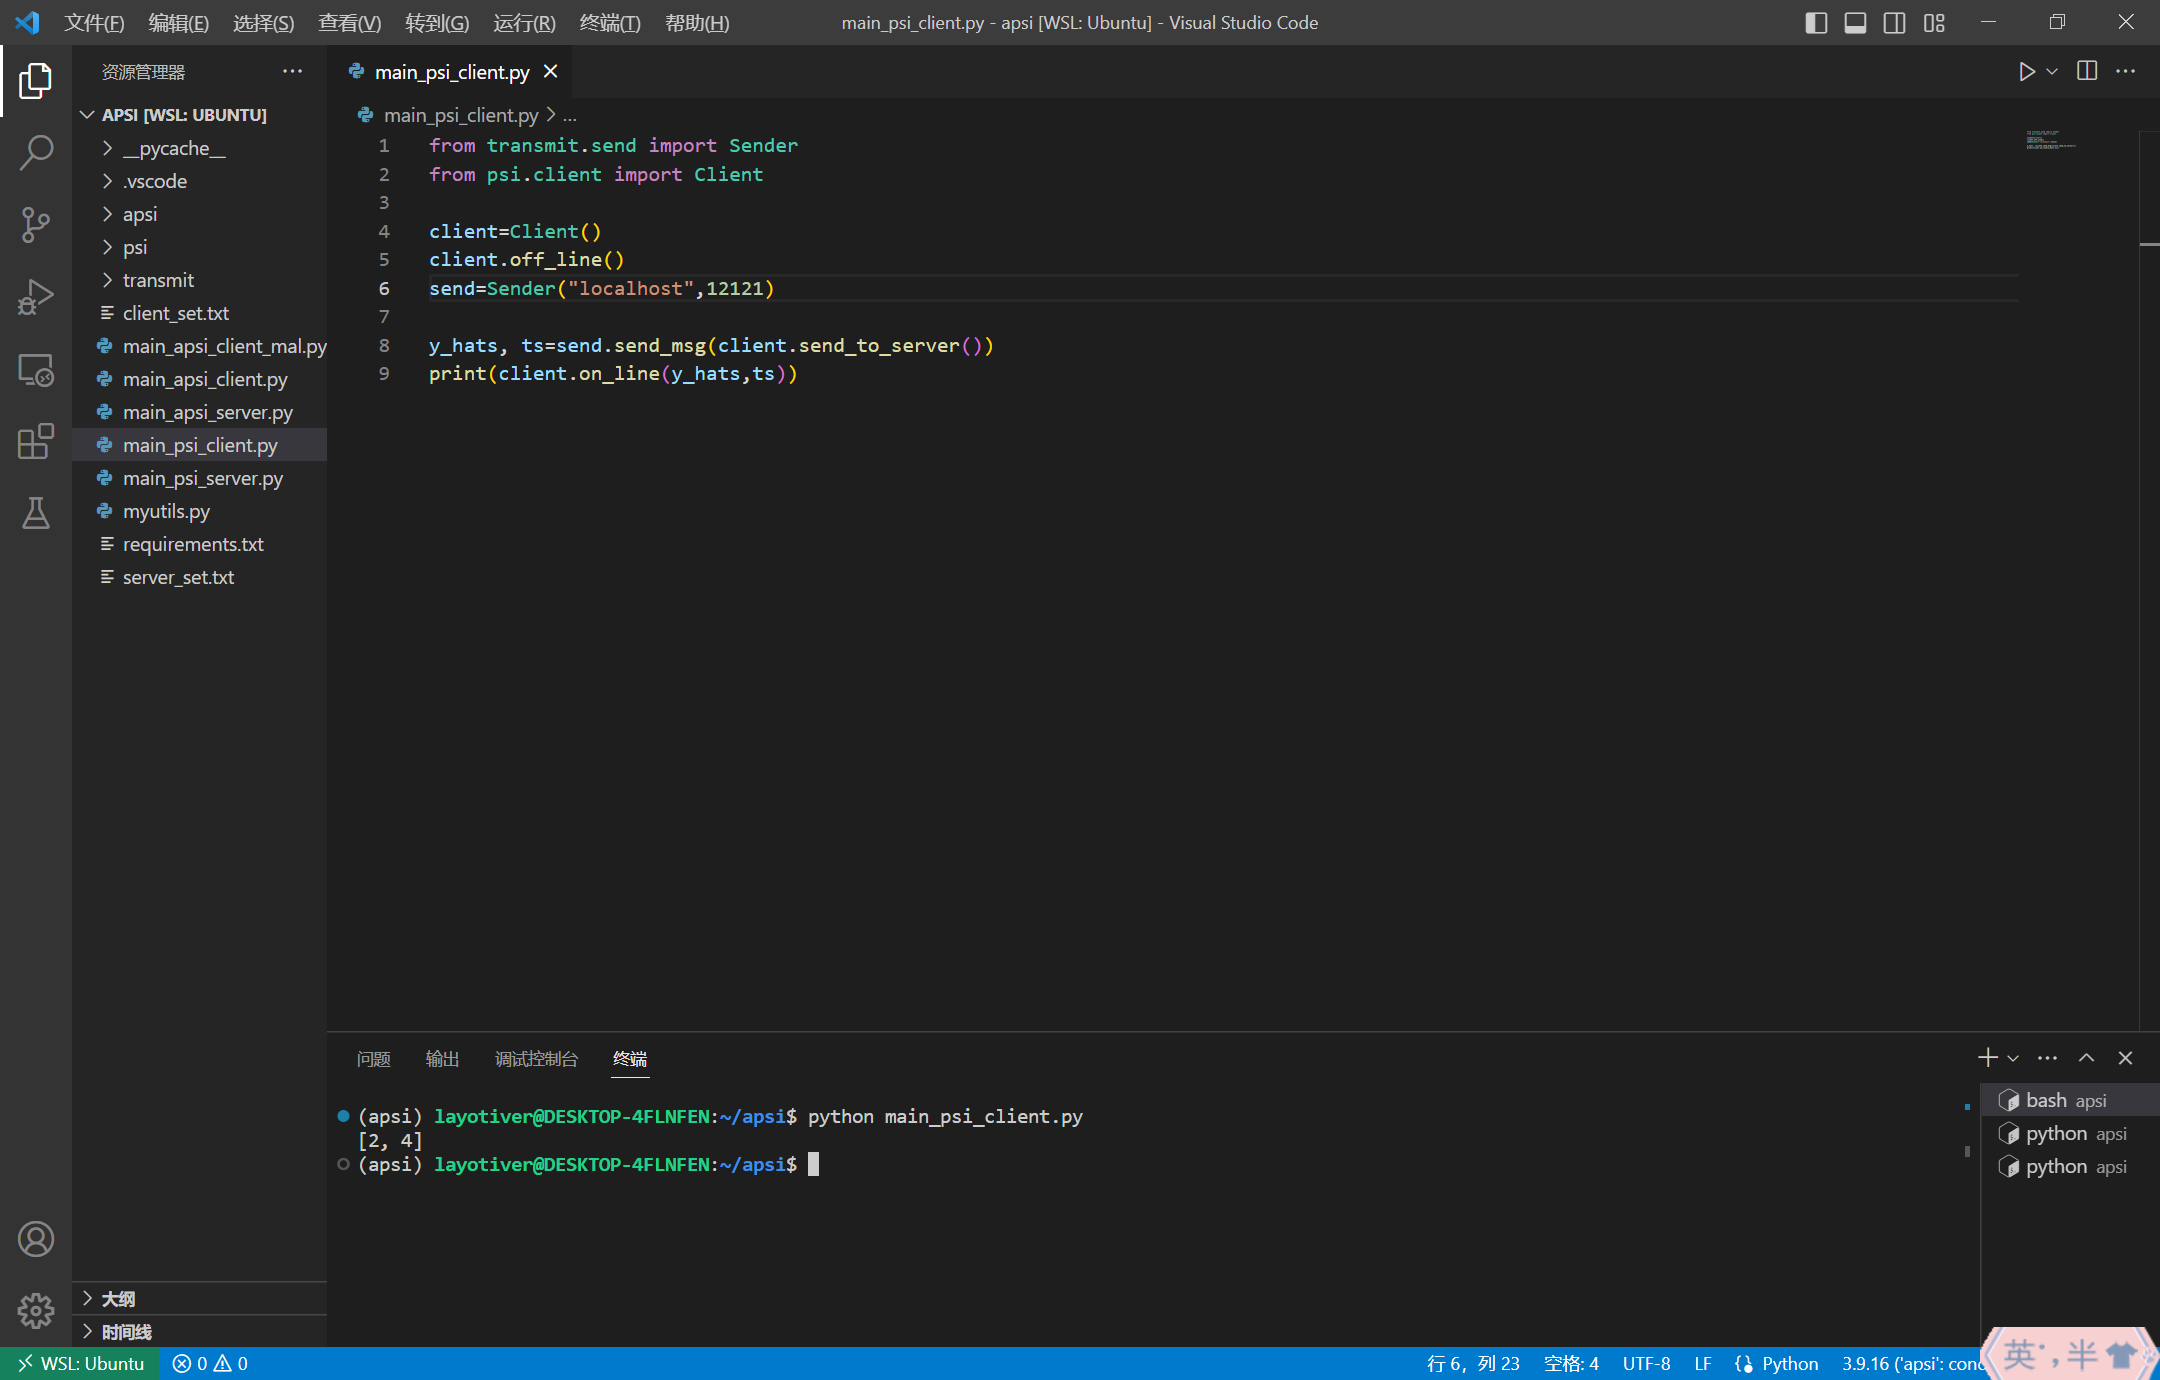
\includegraphics[width=17cm]{experiment0}
    \caption{Blind RSA-based PSI Protocol with linear complexity}
    \label{fig:experiment0}
\end{figure}

\section{APSI protocol}
De Cristofaro等人的PSI协议无法验证客户端的隐私集合的真实性。比如,客户端可以谎称自己的集合里有单词departure(实际上并没有),经过上述PSI协议,最后客户端能够知道服务器端是否有departure这个单词。因此我们需要授权的隐私集合求交(APSI)。我们实现了基于可信第三方证书的APSI,客户端的每个元素都带有CA的证书。

\subsection{Normal case}
我们在\textit{apsi}包里实现了基于证书的PSI协议,这包里同样有\textit{Client}和\textit{Server}类。另外,\textit{apsi}包里还有一个\textit{CertificateAuthority}类,用于给客户端的元素颁发证书。

同样的,运行\textit{main\_apsi\_server.py}后,服务端程序启动。服务端会先进行\textit{off\_line}操作,然后监听本地的12122端口,接收来自客户端的APSI请求。接着运行\textit{main\_apsi\_client.py},客户端先进行\textit{off\_line}操作,这里客户端的\textit{off\_line}操作需要传入一个CA实例用于颁发证书。之后客户端按照协议将需要传输的数据发送到本地的12122端口。服务器收到数据后先进行证书验证。证书验证无误后,服务器端便按照协议进行数据处理,最后将处理过的数据返回给客户端。客户端收到数据后也进行\textit{on\_line}部分的操作,最后算出双方共有的集合元素。若证书验证错误,则客户端会收到服务器端的报错信息。

运行\textit{main\_apsi\_client.py}后,控制台打印出\textit{2,4},代表计算出隐私集合里第2个和第4个元素为共有的元素,结果正确,参见图\ref{fig:experiment1}。
\begin{figure}[h]
    \centering
    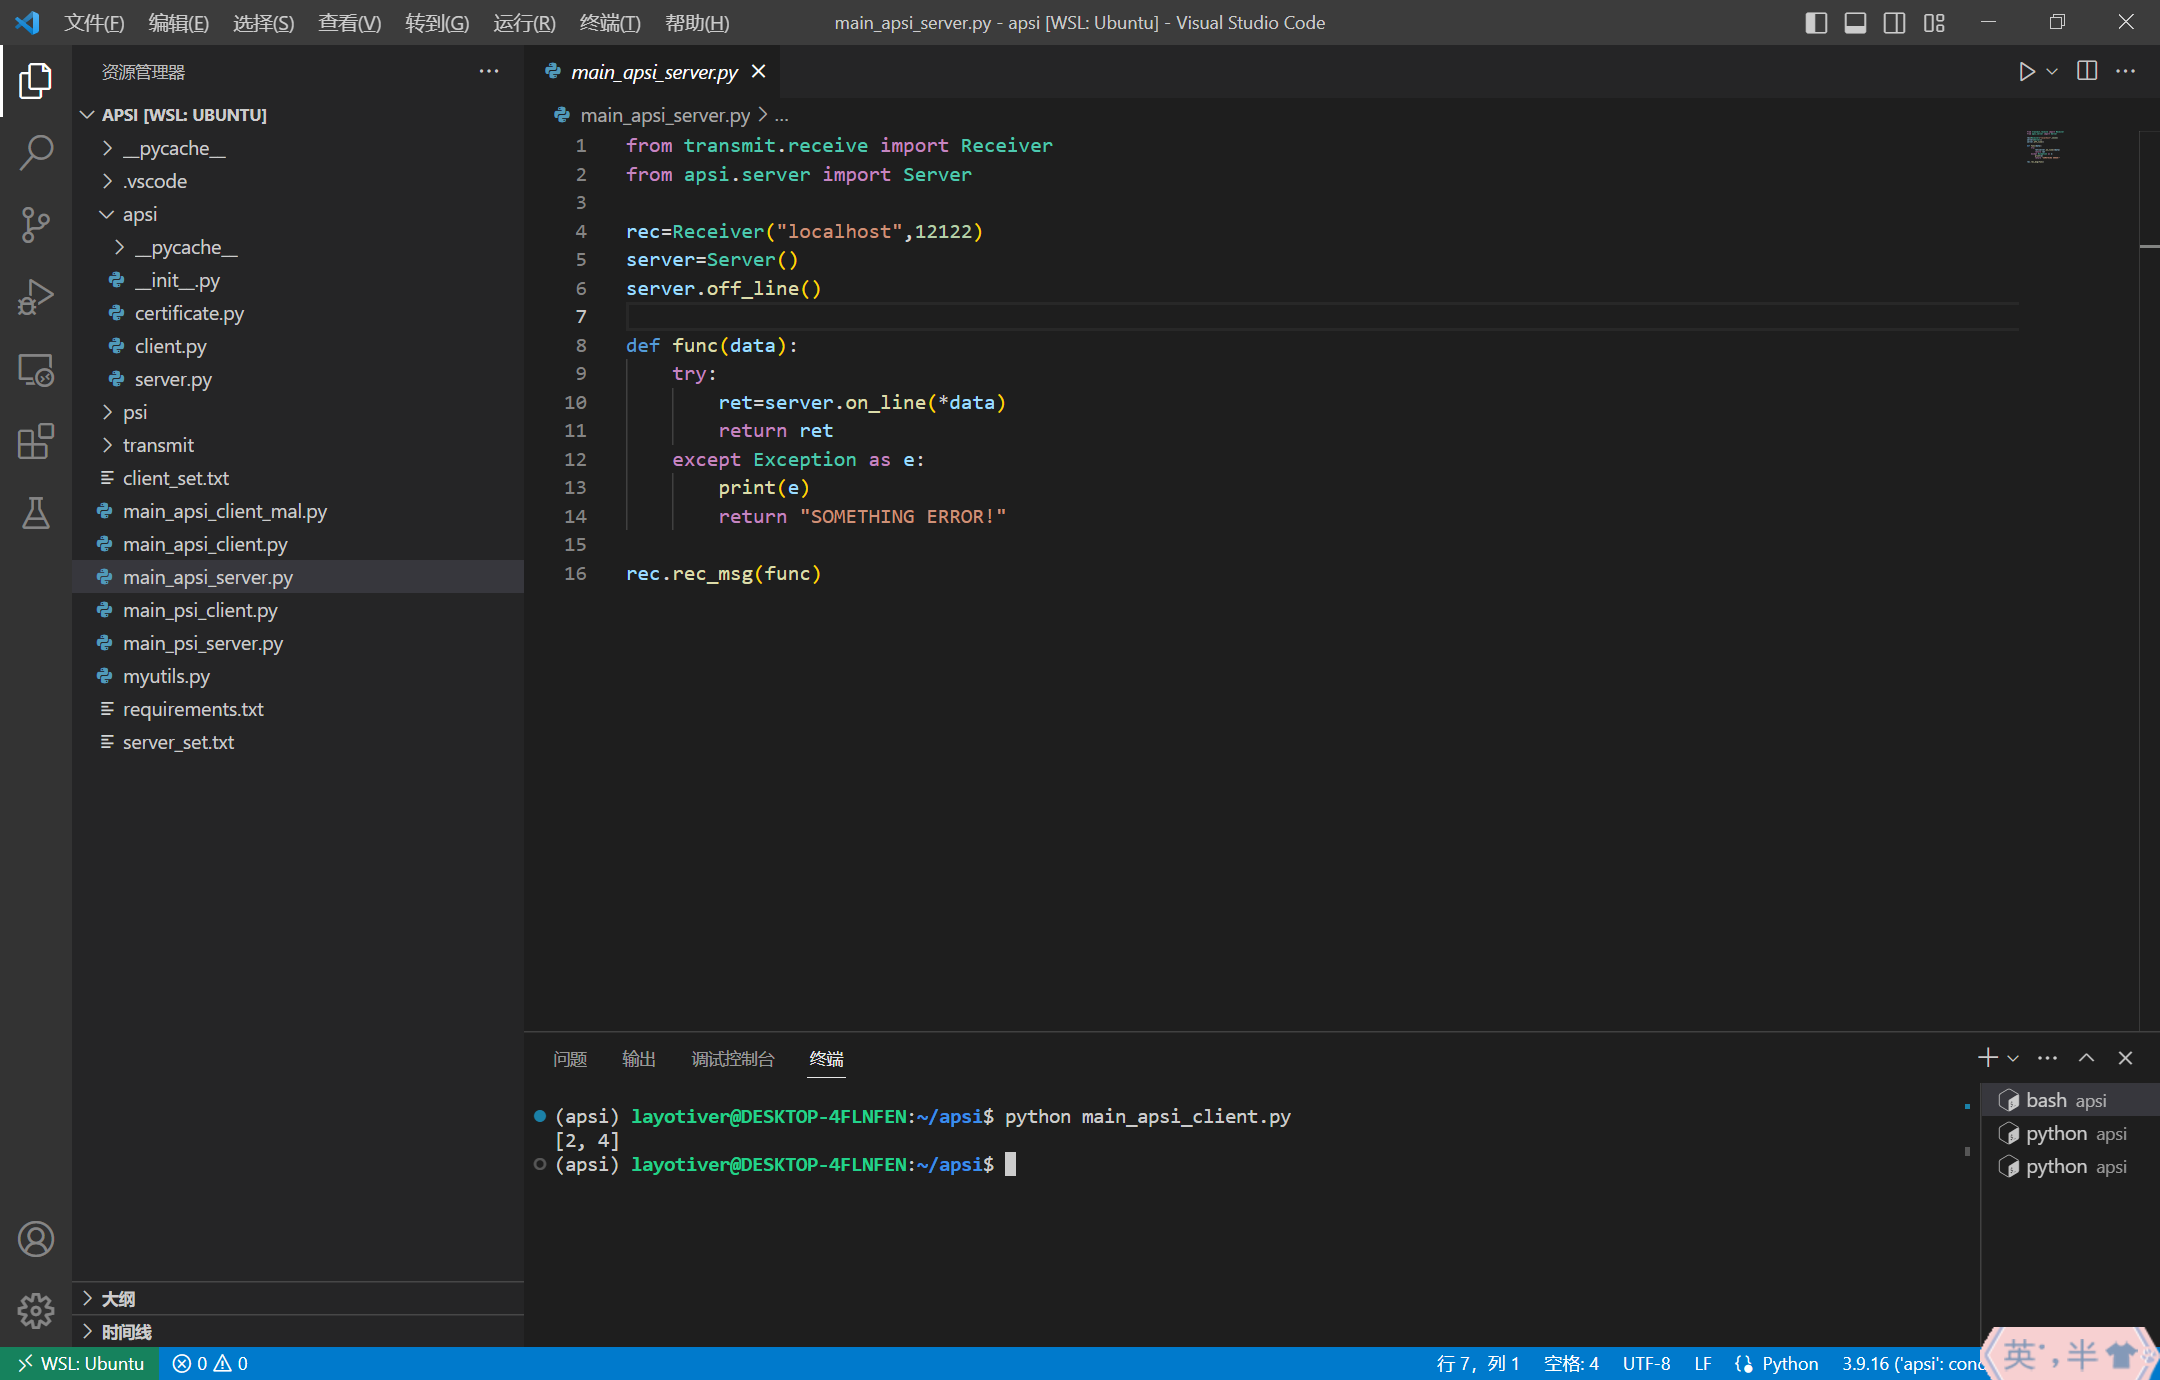
\includegraphics[width=17cm]{experiment1}
    \caption{Blind RSA-based APSI Protocol with linear complexity: Normal}
    \label{fig:experiment1}
\end{figure}


\subsection{Malicious case}
我们设计了客户端带上伪造证书的情况,测试服务器能否检测到证书造假。

运行\textit{main\_apsi\_client\_mal.py},此时客户端的\textit{off\_line}操作传入的CA实例为None,客户端会生成一份全为0的假证书。同样将这些信息发送给服务器,并打印服务器的返回信息。控制台输出-1,即设定了服务器报错信息,测试成功,参见图\ref{fig:experiment2}。
\begin{figure}[h]
    \centering
    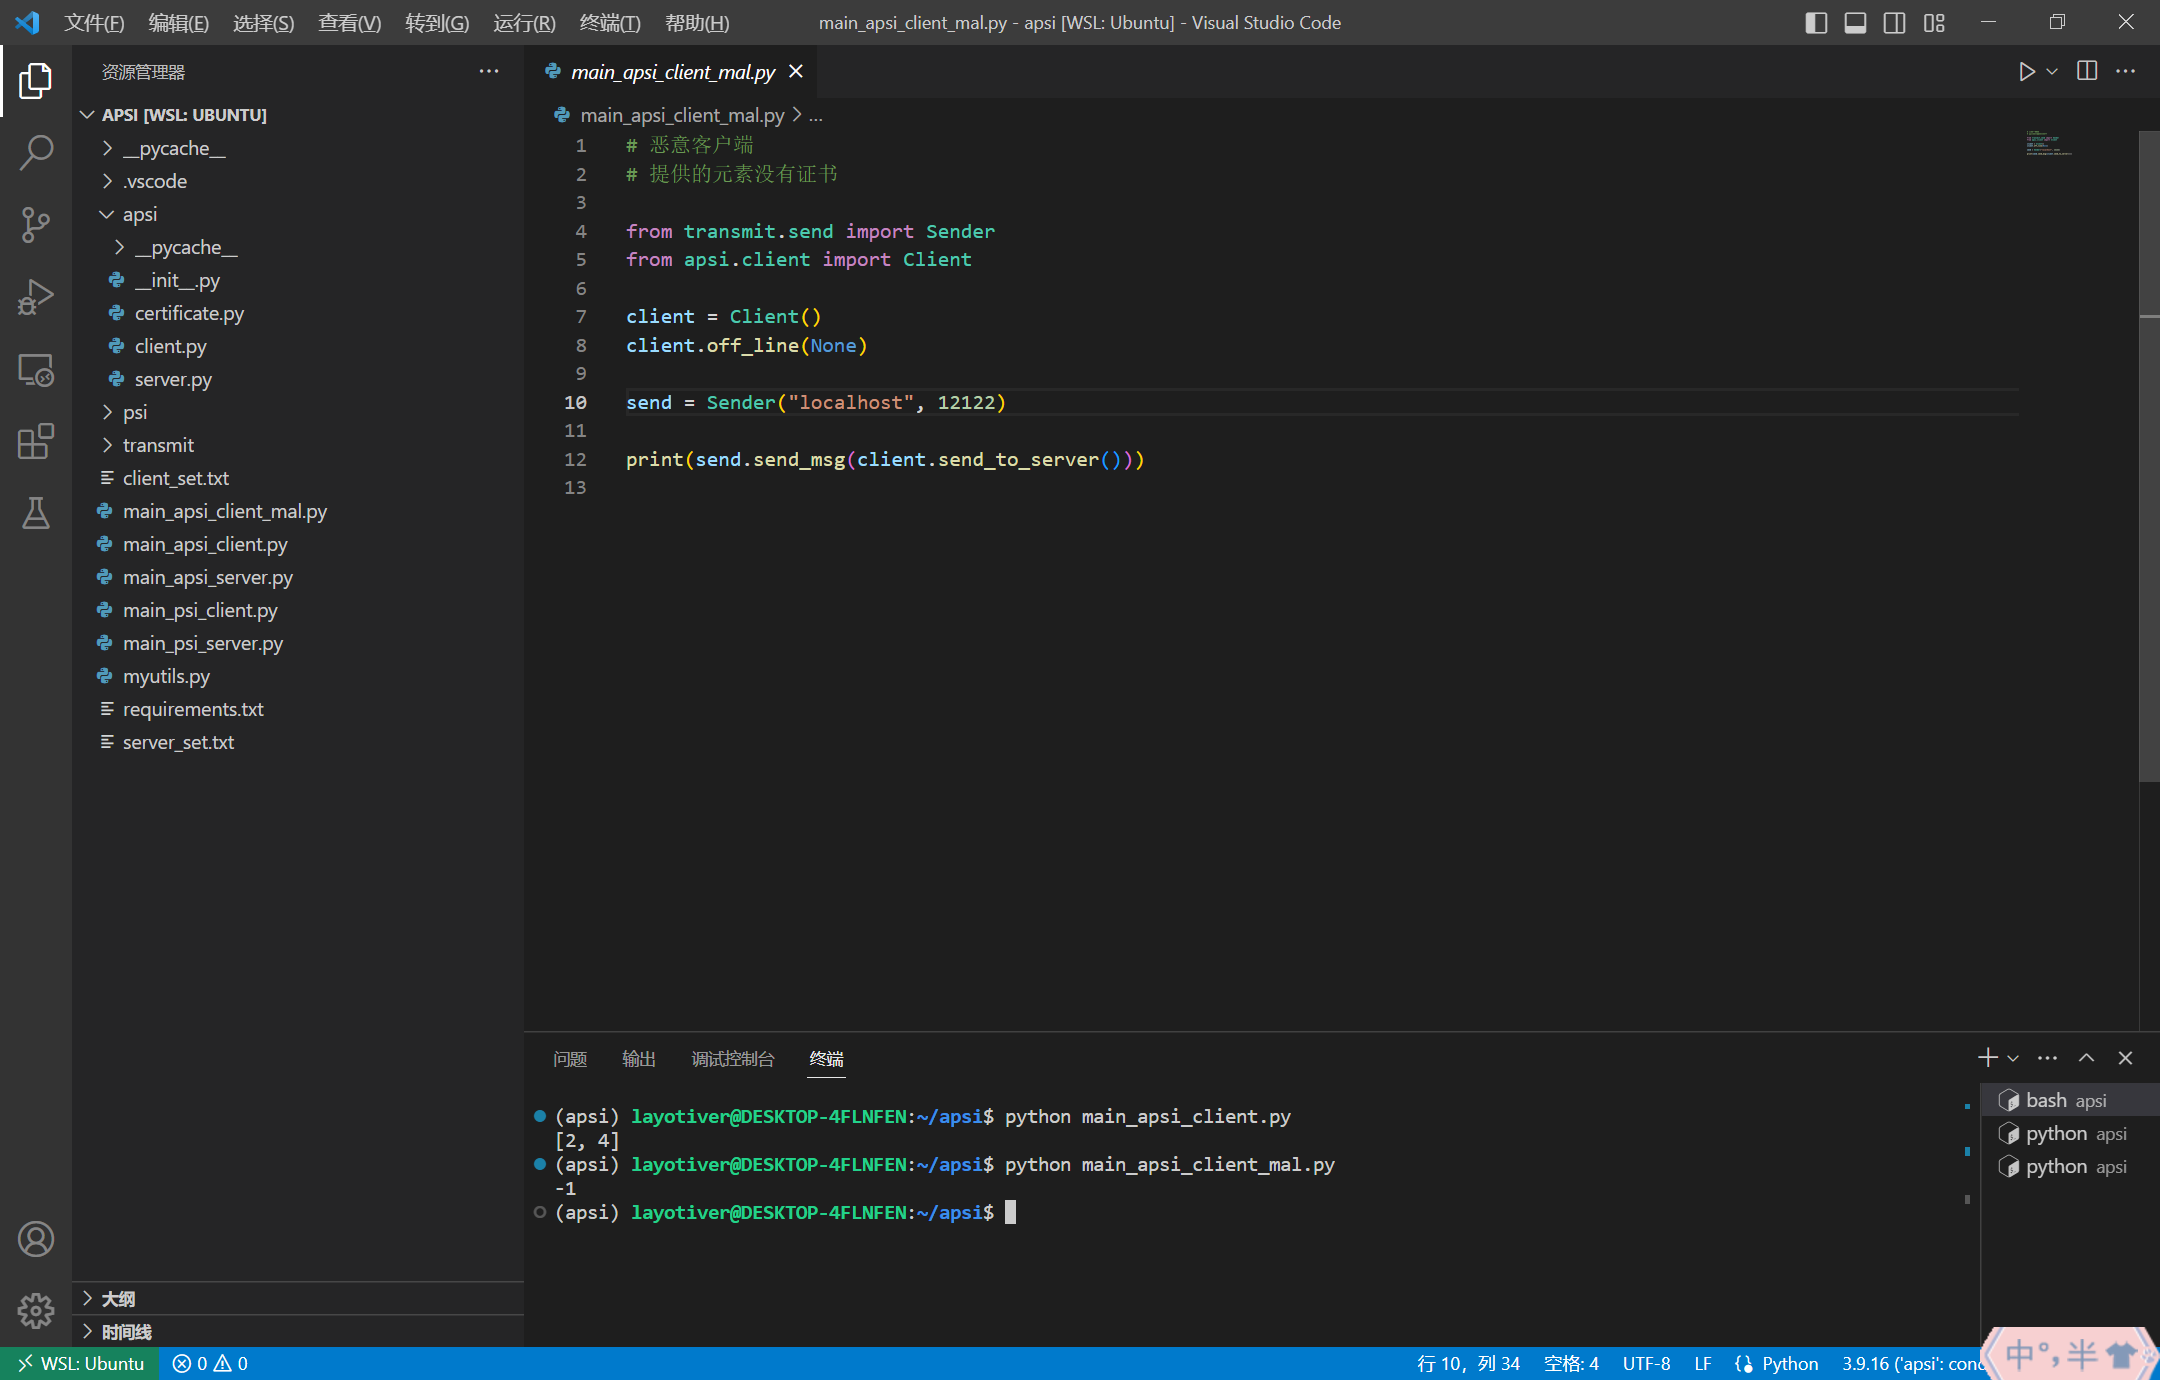
\includegraphics[width=17cm]{experiment2}
    \caption{Blind RSA-based APSI Protocol with linear complexity: Malicious}
    \label{fig:experiment2}
\end{figure}